\section{\system\ Architecture}
\label{sec:architecture}

\subsection{System context}

\begin{figure}[H]
\centering
\IfFileExists{../figures/fig1_system_overview.png}
  {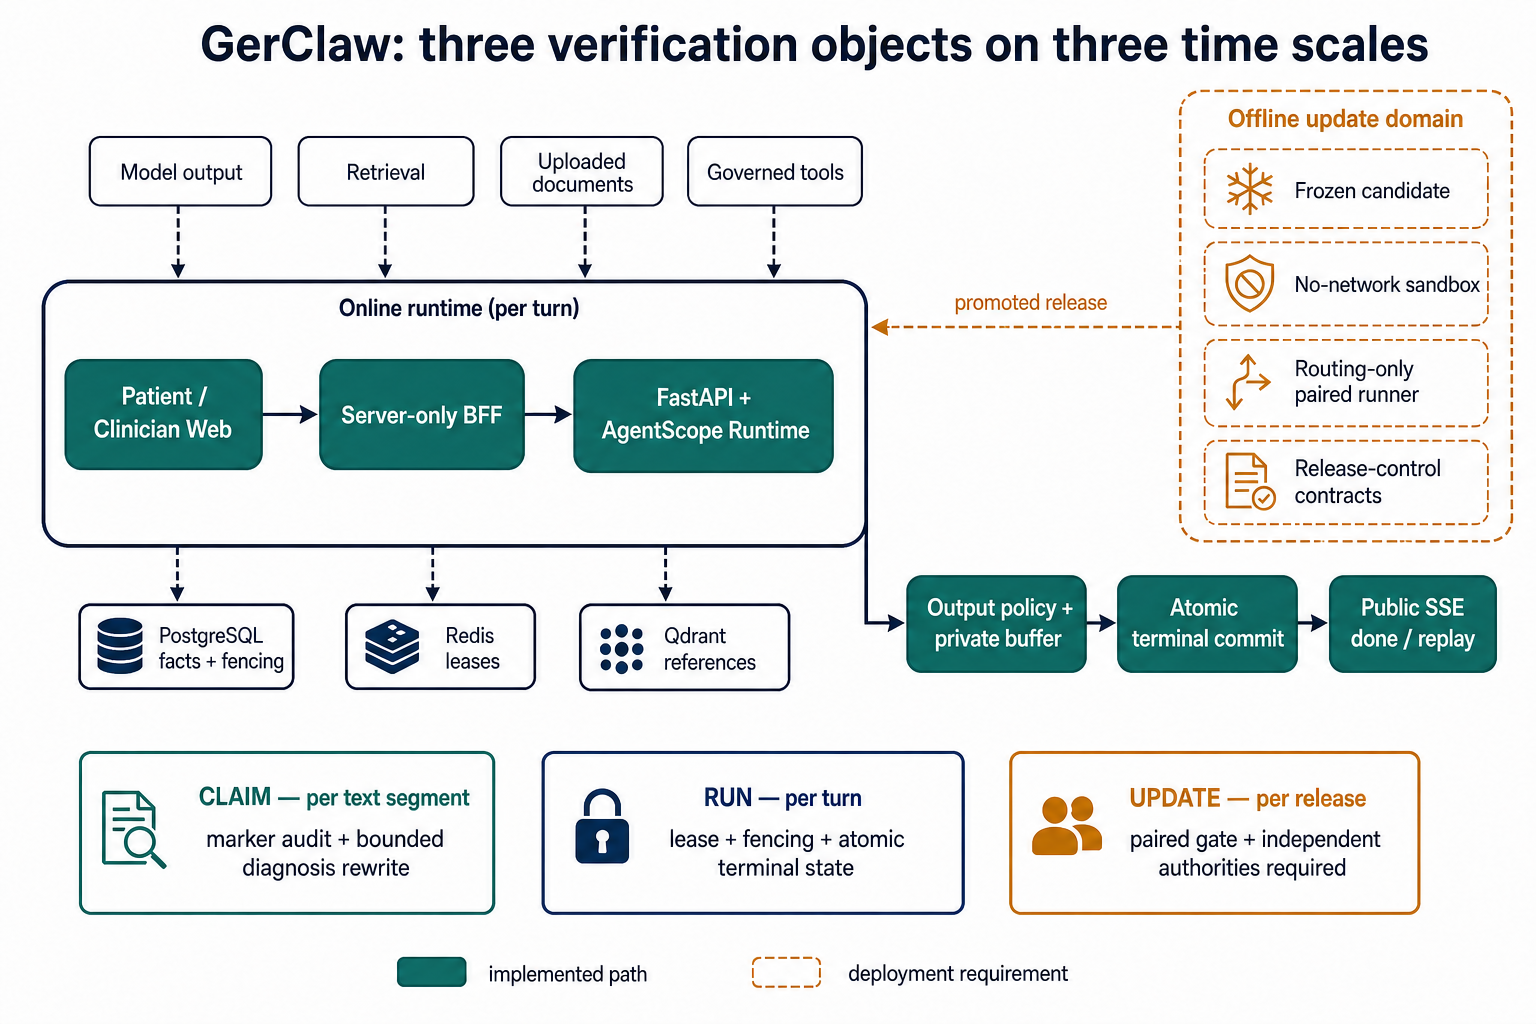
\includegraphics[width=\textwidth]{../figures/fig1_system_overview.png}}
  {\placeholderfigure{3.1cm}{Figure 1 placeholder: GerClaw system overview and
  claim, run, and update verification boundaries.}}
\caption{\system\ separates three verification objects and time scales rather
than a serial pipeline: segments are audited during generation, terminal state
is committed per run, and candidates are evaluated in an offline update
domain.  ``Verified'' denotes the named software property, never clinical
correctness.}
\label{fig:overview}
\end{figure}

\system\ separates a Web/BFF access plane, a FastAPI and AgentScope execution
plane, and durable/coordination stores (Figure~\ref{fig:overview}).  The
browser receives versioned JSON and server-sent events (SSE) but no provider,
database, or vector-store credentials.  PostgreSQL is the encrypted fact
source; Redis coordinates leases, cancellation, and short-lived guards; and
Qdrant stores retrieval and memory references that resolve back to durable
records.  Model, search, speech, parsing, embedding, and reranking providers
sit behind server-side adapters.

Each turn creates an isolated agent state.  An authenticated tenant, actor,
session, and trace scope determines which memory, documents, skills, and
tools can be composed.  The bounded ReAct loop defaults to six iterations.
Model fallback is allowed only before visible text or a tool call; the runtime
fails closed rather than splice outputs from two models after a partial
stream.

\subsection{Claim and evidence path}

\begin{figure}[H]
\centering
\IfFileExists{../figures/fig2_claim_evidence.png}
  {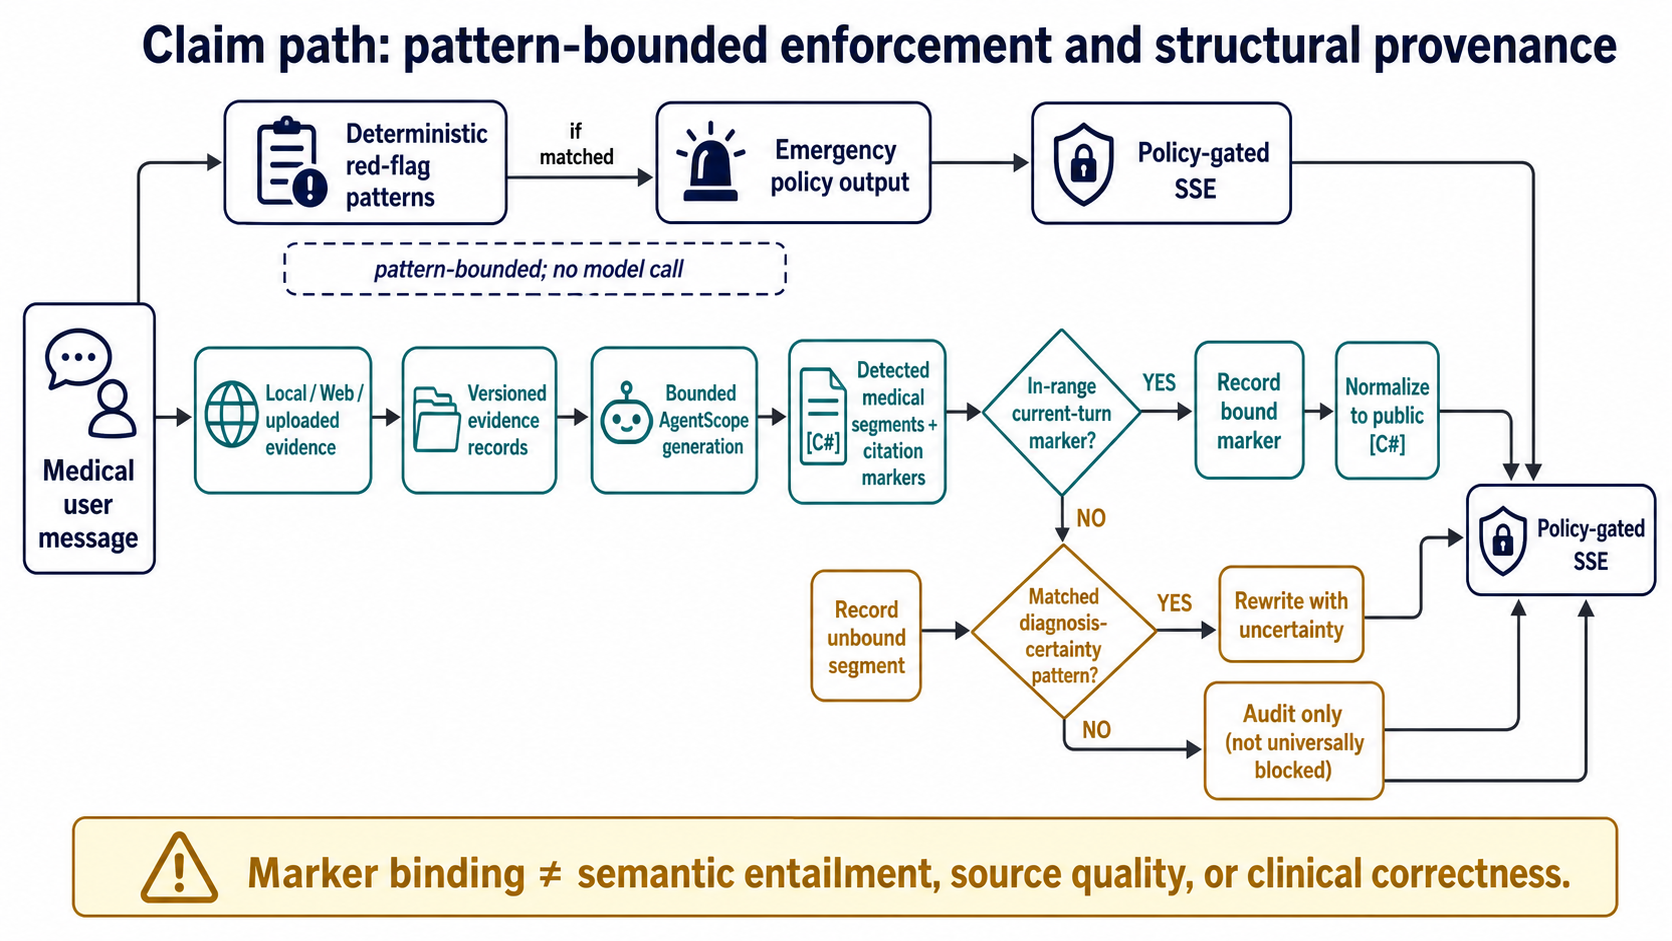
\includegraphics[width=\linewidth]{../figures/fig2_claim_evidence.png}}
  {\placeholderfigure{4.2cm}{Figure 2 placeholder: deterministic emergency
  branch and claim--evidence binding.}}
\caption{The claim path separates pattern-bounded escalation from
model-mediated generation.  It audits marker structure and rewrites only
matched unbound diagnosis-certainty patterns; other unbound segments are
recorded but not universally blocked.}
\label{fig:claims}
\end{figure}

Figure~\ref{fig:claims} shows two paths.  First, a deterministic red-flag
policy can short-circuit recognized emergency inputs, emit urgent-action
guidance, attach the uniform medical disclaimer, and close the turn without
calling a model.  This path is intentionally narrow: pattern coverage is not
equivalent to comprehensive triage.

Second, ordinary medical inputs can invoke local retrieval, governed Web
search, and tenant-scoped uploaded evidence.  Evidence responses are parsed
into versioned records before reaching the agent.  Retrieved or uploaded
content is treated as data and cannot grant tool authority.  After generation,
the output path normalizes in-range current-turn evidence markers and records
detected medical segments as bound or unbound.  For a narrow set of
deterministic diagnosis-assertion patterns, an unbound segment is rewritten
with uncertainty; other unbound clinical statements are currently audited but
not universally blocked.  The mechanism checks marker structure, not
entailment.  Patient-facing actionable conclusions receive one concise review
notice; clinician-facing output is not mechanically suppressed.

\subsection{Transactional run lifecycle}

\begin{figure}[H]
\centering
\IfFileExists{../figures/fig3_transactional_run.png}
  {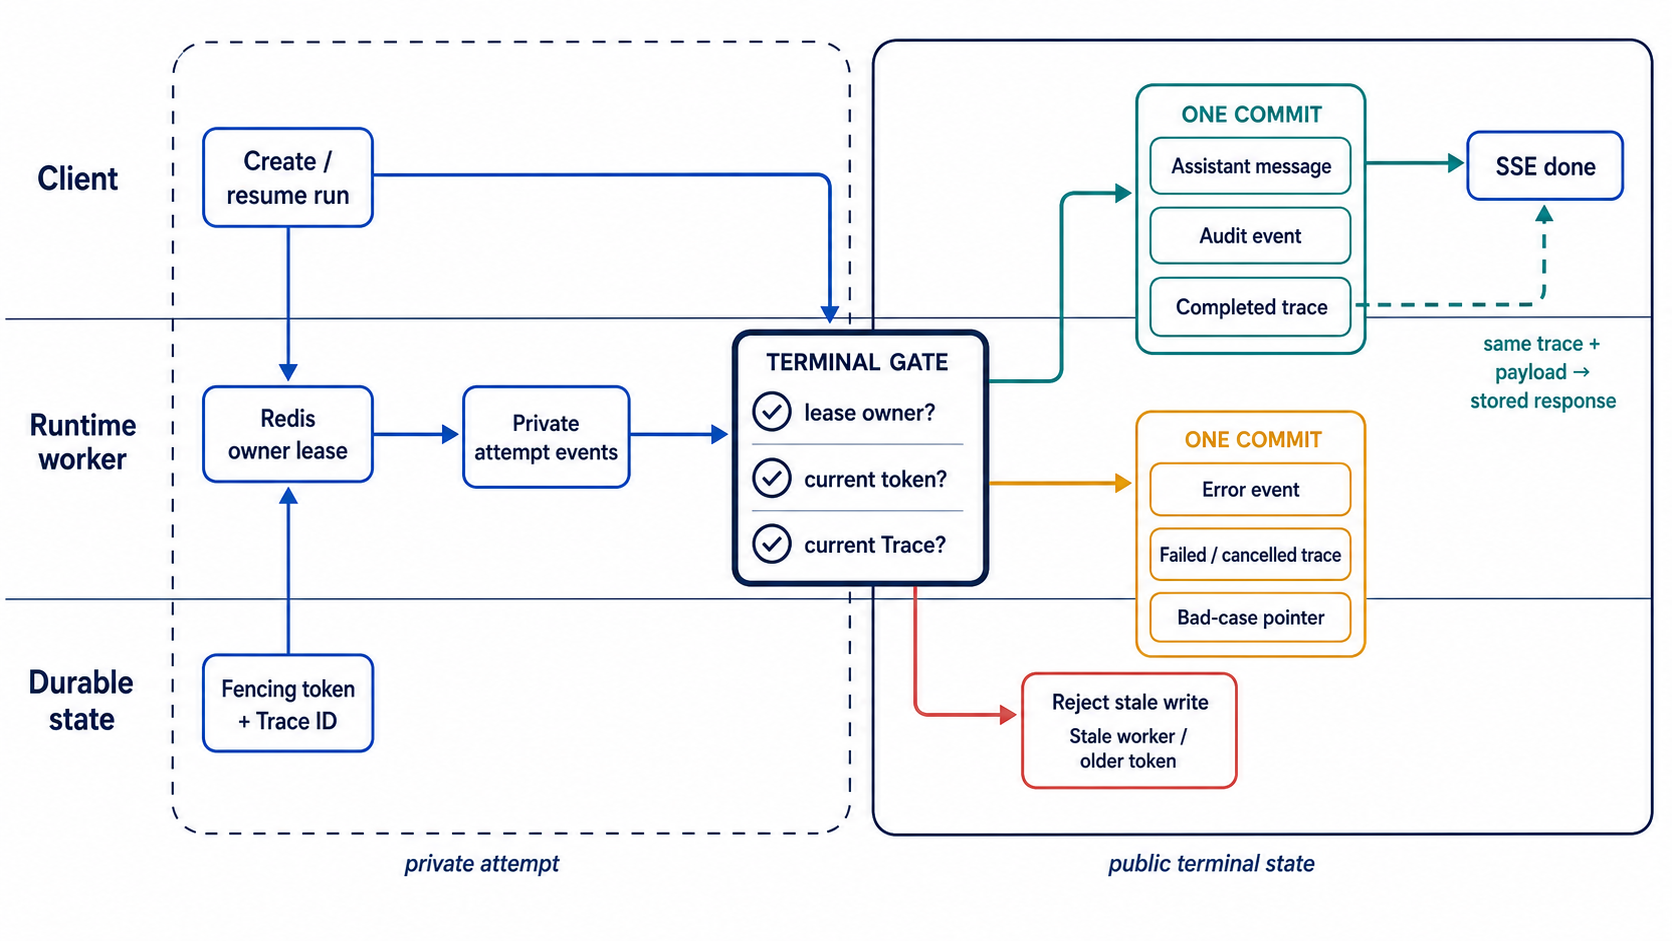
\includegraphics[width=\linewidth]{../figures/fig3_transactional_run.png}}
  {\placeholderfigure{4.0cm}{Figure 3 placeholder: lease, fencing, private
  attempts, and atomic terminal commit.}}
\caption{Run verification.  A Redis lease serializes the common case; a
monotonic PostgreSQL fencing token rejects a stale owner.  Success or failure
becomes public through one terminal transaction, and \texttt{done} follows
the commit.}
\label{fig:run}
\end{figure}

A random owner token leases a session while PostgreSQL assigns a monotonic
fencing token to each attempt.  The new owner writes its token and trace ID
before loading bounded history.  Before any terminal write, it renews and
compares the Redis owner and locks the corresponding PostgreSQL session row to
verify the token and trace.

On success, the assistant message, audit event, and completed trace share one
transaction.  On failure or cancellation, the stable public error, failed or
cancelled trace, and de-identified bad-case pointer share a corresponding
transaction.  Rollback prevents a partial terminal state.  Only after commit
does the runtime emit \texttt{done}; a completed retry with the same trace and
payload returns the stored encrypted response without a second model call.
This design does not make Redis a fact source: the database record remains
authoritative when leases expire or processes disappear.

\subsection{Governed offline evolution}

\begin{figure}[H]
\centering
\IfFileExists{../figures/fig4_offline_evolution.png}
  {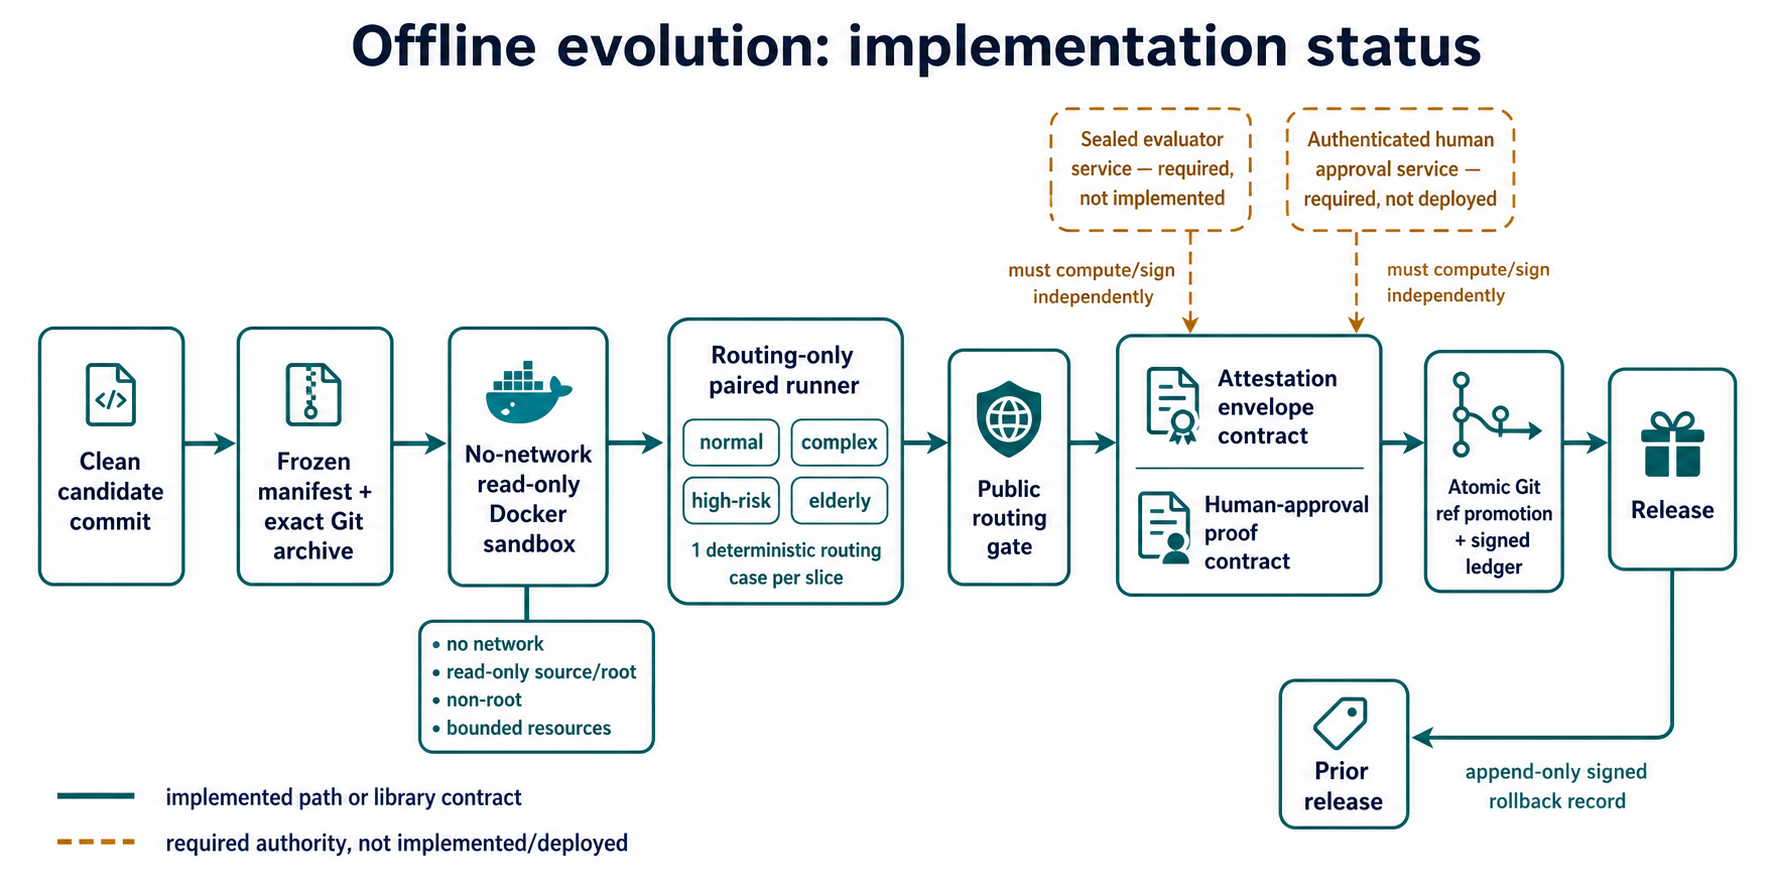
\includegraphics[width=\textwidth]{../figures/fig4_offline_evolution.png}}
  {\placeholderfigure{3.6cm}{Figure 4 placeholder: frozen candidate,
  restricted sandbox, paired and sealed evaluation, human approval, atomic
  promotion, and signed rollback.}}
\caption{Update contracts and implementation status.  Solid components are
implemented library or routing-runner paths; dashed authorities are required
for a complete deployment but are not implemented or deployed in this work.}
\label{fig:evolution}
\end{figure}

The evolution controller is an operator-run application outside the
production API image.  It accepts a clean candidate commit, freezes the
committed diff and modes, and binds every changed path to an allowed
object-kind policy.  Execution uses an exact Git archive in a
content-addressed, preinstalled Docker image with no network, a read-only root
and source, non-root identity, isolated temporary storage, bounded resources,
and verified cleanup.  The live worktree, source repository, Docker socket,
credentials, release references, and hidden tests are not mounted.

The only concrete paired runner currently accepts
\texttt{routing.strategy}.  Baseline and candidate use the same
evaluation-profile digest on four deterministic cases---one each for normal,
complex, high-risk, and elderly slices---and verify the intended router module
was activated.  This demonstrates a narrow execution path, not general agent
quality or subgroup coverage.

The control library defines two additional artifact contracts.  An
attestation envelope binds declared sealed-gate facts to an evaluator key, and
an approval envelope binds an exact candidate, reports, ticket, and trusted
time to an Ed25519 key.  The repository does not contain the independent
hidden-case runner that computes those sealed facts, and the approval signer
is a package class rather than a deployed authenticated service.  A complete
\updategate\ deployment must supply and isolate both authorities.  The
promotion library re-verifies artifacts and moves release and ledger
references in one Git reference transaction; rollback appends a signed
history entry instead of erasing the prior release.
